\documentclass[12pt, letterpaper]{article}

\usepackage[utf8]{inputenc}
\usepackage[T1]{fontenc}
\usepackage[spanish]{babel}
\usepackage{sourcesanspro}
\renewcommand{\familydefault}{\sfdefault}
\usepackage[margin=2.5cm]{geometry}
\usepackage{graphicx}
\usepackage{setspace}
\usepackage{tabularx}
\usepackage{float} % Agregado para usar [H] en las figuras

\setlength{\parindent}{1.5em}
\setlength{\parskip}{0.4em}
\setstretch{1.5}

\begin{document}

% ================= PORTADA =================
\begin{titlepage}
    \begin{center}
        \begin{minipage}[c]{0.18\textwidth}
            \centering
            
\includegraphics[height=2.0cm]{UC_logo.png}
        \end{minipage}%
        \begin{minipage}[c]{0.64\textwidth}
            \centering
            \normalsize Universidad de Carabobo. \\
            \normalsize Facultad Experimental de Ciencias y Tecnología. \\
            \normalsize Arquitectura del Computador. \\
            \normalsize Sección 1.
        \end{minipage}%
        \begin{minipage}[c]{0.18\textwidth}
            \centering
            
\includegraphics[height=2.0cm]{FACYT_logo.png}
        \end{minipage}
        
        \vspace{5cm}
        \Huge \textbf{Informe.} \\[0.7cm]
        \Huge \textbf{Práctica de Laboratorio 2.}

    \end{center}
    \vfill
    \begin{minipage}[t]{0.5\textwidth}
        \large \textbf{Integrantes:}\\
        Penélope Robledo, C.I. 32.482.938.\\
        Nathalia Noguera, C.I. 32.756.046.
    \end{minipage}
    \hfill
    \begin{minipage}[t]{0.5\textwidth}
        \raggedleft
        \large \textbf{Profesor:}\\
        José Canache.
    \end{minipage}
    \vspace{1.5cm}
    \begin{center}
        \large Naguanagua, Agosto de 2026.
    \end{center}
\end{titlepage}

\newpage

\section*{Introducción}

La presente práctica tiene como objetivo principal el estudio e implementación de algoritmos de ordenamiento en lenguaje ensamblador para la arquitectura MIPS de 32 bits, utilizando el simulador MARS como entorno de desarrollo y depuración. En este contexto, se desarrollaron e implementaron dos algoritmos clásicos: Quicksort, en su versión recursiva, y Mergesort, en su versión iterativa, con el fin de analizar de manera comparativa su comportamiento a bajo nivel.

A lo largo del desarrollo se examinaron aspectos fundamentales de la arquitectura RISC de MIPS, entre los que destacan el uso de registros según la convención de llamada, el impacto del tráfico de memoria frente al uso de registros, las estructuras de control, la complejidad computacional de ambos algoritmos y el camino de datos de las instrucciones. Asimismo, se emplearon de forma sistemática las herramientas de depuración disponibles en MARS (Ejecución paso a paso, ventana de Registros y visualización del datapath mediante MIPS X-Ray) para verificar la correcta ejecución de los programas y comprender el flujo interno del procesador.

Las implementaciones fueron sometidas a diversas pruebas con arreglos de distintos tamaños, valores grandes y números negativos, con el propósito de evaluar su robustez y comportamiento ante diferentes condiciones de entrada. A través de este proceso se busca no solo lograr el ordenamiento correcto de los datos, sino también profundizar en la comprensión de cómo las decisiones algorítmicas se traducen en operaciones de bajo nivel y de qué manera las características de la arquitectura MIPS influyen en el rendimiento, la eficiencia y la fiabilidad de las soluciones implementadas.\\

\section*{1. ¿Qué diferencias existen entre registros temporales (\$t0–\$t9) y registros guardados (\$s0–\$s7) y cómo se aplicó esta distinción en la práctica?}

En la arquitectura MIPS32, el banco de registros no se comporta como un espacio uniforme en el que cualquier valor puede almacenarse indistintamente, sino que responde a una convención de registros conocida como convención de llamada (calling convention), que reparte la responsabilidad de preservar cada registro entre quien invoca una subrutina y quien es invocado. Los registros temporales (\$t0–\$t9) y los registros guardados (\$s0–\$s7) comprenden las dos categorías centrales de dicha convención. Esta distinción está lejos de ser un simple formalismo, ya que condicionó directamente las decisiones de diseño tomadas en ambos algoritmos de ordenamiento implementados.

Los registros \$t0–\$t9 son registros temporales y se consideran de tipo caller-saved, es decir, protegidos por quien realiza la llamada. Ninguna función o subrutina invocada mediante la instrucción jal tiene la obligación de conservar el contenido que estos registros poseían antes del salto, siendo que en el caso de que dicho valor sea necesario después del retorno, es responsabilidad exclusiva de la función que llama resguardarlo, generalmente en la pila, antes de ejecutar jal. Por su naturaleza, estos registros están pensados para cálculos intermedios de vida corta, que nacen y se consumen dentro del mismo bloque de instrucciones sin necesidad de sobrevivir a un salto.

En cambio, los registros \$s0–\$s7 son callee-saved, protegidos por quien es llamado, y cualquier función que decida emplear alguno de ellos para una variable que deba permanecer válida durante toda su ejecución, incluso a través de llamadas internas a otras partes del código, adquiere el compromiso de guardar su valor original inmediatamente después de reservar espacio con addi \$sp, \$sp, -n y de restaurarlo justo antes de liberar este espacio y ejecutar jr \$ra.

Esta distinción se aplicó de manera muy concreta en ambos programas, y el ejemplo más claro se encuentra en la relación entre main y leer\_arreglo, presente de forma idéntica en los dos algoritmos. En el main, la cantidad de elementos leída por teclado se guarda mediante move \$s0, \$v0, y ese mismo registro \$s0 se reutiliza más adelante para armar los parámetros de Quicksort o Mergesort y de imprimir\_arreglo. Sin embargo, dentro de leer\_arreglo, \$s0 se emplea nuevamente, esta vez como contador del bucle ciclo\_lectura (move \$s0, \$zero; addi \$s0, \$s0, 1). Si leer\_arreglo no hubiera preservado \$s0 mediante sw \$s0, 0(\$sp) al entrar y lw \$s0, 0(\$sp) al salir, el valor de la cantidad de elementos que main había guardado se habría perdido totalmente al retornar, arrastrando un error en cascada hacia el resto del programa. Este caso demuestra la razón de ser de la convención callee-saved, ya que sin ella, dos funciones no relacionadas entre sí no podrían compartir de forma segura el mismo espacio de registros.

Otro ejemplo que se presenta, aunque de sentido opuesto, aparece en partition. Allí, el índice i (guardado en \$t8) y el valor del pivote (guardado en \$t9) deben sobrevivir a la llamada jal swap dentro del ciclo ciclo\_j, a pesar de hallarse en registros temporales que por convención no son resguardados. La solución adoptada en el código se basa en en guardarlos manualmente en la pila justo antes de la llamada (sw \$t8, 4(\$sp) y sw \$t9, 0(\$sp)) y recuperarlos inmediatamente después (lw \$t9, 0(\$sp) y lw \$t8, 4(\$sp)), tratándolos con estos fines como si fueran registros guardados. Por lo tanto, la distinción \$t/\$s no es una restricción física del hardware, sino una convención de software, porque el programador puede usar cualquier registro para cualquier propósito, pero al hacerlo fuera de la convención asume manualmente la carga de protegerlo, tal como ocurre aquí.

En Quicksort, los registros \$s0 (arreglo v), \$s1 (inicio) y \$s2 (fin) se mantienen a lo largo de toda la ejecución de partition, mientras que en la función Quicksor tse añade \$s3 para almacenar el índice del pivote devuelto por partition, valor que debe permanecer intacto a través de las dos llamadas recursivas subsiguientes (jal Quicksort). De no emplear un registro guardado para este propósito, cualquier llamada recursiva interna destruiría su contenido, ya que las subrutinas invocadas hacen uso libre de los registros \$t. En Mergesort ocurre algo parecido, debido a que los registros \$s0 (base del arreglo), \$s1 (n), \$s2 (ancho de bloque o tam) y \$s3 (índice de inicio de bloque, izq) deben mantenerse válidos a través de múltiples llamadas jal merge anidadas dentro de los bucles ciclo\_tam y ciclo\_izq, mientras que los registros \$t0–\$t7 se reutilizan libremente en cada iteración para calcular los límites medio y derecha, precisamente porque esos valores se recalculan por completo en cada iteración y não necesitan sobrevivir a una llamada.

Vale la pena señalar además, un detalle en leer\_arreglo e imprimir\_arreglo. El registro \$t0, empleado como índice que recorre las posiciones del arreglo, también debe conservar su valor a través de cada syscall (li \$v0, 4/5 seguido de syscall), sin que exista ninguna garantía por parte de la convención de llamada que lo proteja. Que el código funcione correctamente depende en este caso de que el manejador de syscalls de MARS no modifique los registros temporales del programa, un comportamiento propio del simulador y no un respaldo de la arquitectura. Si ocurriera una excepción o interrupción real que sí alterara el banco de registros, este diseño resultaría frágil.\newpage

\section*{2. ¿Qué diferencias existen entre los registros \$a0–\$a3, \$v0–\$v1, \$ra y cómo se aplicó esta distinción en la práctica?}

Además de los registros temporales y guardados, la convención de llamada de MIPS32 define un tercer grupo de registros especializados exclusivamente en la comunicación entre una función y quien la invoca, que son los registros de argumentos (\$a0–\$a3), los registros de valor de retorno (\$v0–\$v1) y el registro de dirección de retorno (\$ra). A diferencia de \$t y \$s, cuyo propósito depende de cómo decida usarlos el programador, estos tres grupos tienen un rol fijo dentro del protocolo de llamada, y su aplicación en ambos algoritmos demuestra claramente las diferencias estructurales entre Quicksort y Mergesort.

Los registros \$a0–\$a3 transportan hasta cuatro parámetros al inicio de una función o procedimiento, siguiendo el orden de posiciones en el que se cargan antes del jal. En la práctica, ningún procedimiento de Quicksort necesitó más de tres, porque leer\_arreglo e imprimir\_arreglo reciben la dirección del arreglo (\$a0) y la cantidad de elementos (\$a1), swap recibe el arreglo (\$a0) y dos índices a intercambiar (\$a1, \$a2), partition y Quicksort reciben el arreglo y el rango [inicio, fin] a procesar (\$a0, \$a1, \$a2). En contraste, Mergesort sí requiere los cuatro registros de argumento en su función merge, ya que fusionar dos subarreglos ordenados requiere especificar tres separaciones (izquierda, medio y derecha) además de la base del arreglo con las instrucciones move \$a0, \$s0; move \$a1, \$s3; move \$a2, \$t1; move \$a3, \$t3. Mientras que la partición de Quicksort solo necesita un rango, la unión de Mergesort necesita aparte del rango completo el punto exacto donde termina la primera mitad y comienza la segunda, y ese dato hace que se utilicen todos los registros \$a0–\$a3, sin dejar margen para un quinto parámetro sin recurrir a la pila.

El registro \$v0 cumple en este código dos papeles. Por un lado, actúa como selector de servicio del sistema: antes de cada syscall se le asigna el código correspondiente (li \$v0, 4 para imprimir cadena, li \$v0, 5 para leer entero, li \$v0, 1 para imprimir entero, li \$v0, 10 para terminar el programa), y tras una llamada de lectura, el propio \$v0 pasa a contener el valor devuelto, tal como se ve en move \$s0, \$v0 dentro del main o en sw \$v0, 0(\$t0) dentro de ciclo\_lectura. Por otro lado, \$v0 también cumple su función como registro de retorno de una función definida por el programador. En partition, al finalizar, deja en \$v0 el índice donde quedó ubicado el pivote (lw \$v0, 0(\$sp) en la etiqueta fin\_j), valor que Quicksort recoge inmediatamente con move \$s3, \$v0 para construir los límites de sus dos llamadas recursivas. El registro \$v1, por el contrario, no se utiliza en ningún punto de los dos programas, a causa de que ninguna de las funciones definidas necesita devolver un segundo valor al mismo tiempo, de manera que ambos algoritmos se realizaron con retornos de un solo valor.

El registro \$ra por su parte, al ser único, cualquier llamada jal anidada sobrescribe su contenido, de modo que toda función que a su vez realice llamadas internas debe protegerlo explícitamente antes de hacerlo. Esto se cumple en partition (que llama a swap), en Quicksort (que se llama recursivamente a sí misma dos veces y llama a partition) y en Mergesort (que llama a merge repetidamente dentro de sus bucles anidados), donde todas ellas comienzan guardando \$ra en la pila y terminan restaurándolo justo antes de jr \$ra. La única función que no necesita esta protección es swap, que no ejecuta ningún jal en su interior, razón por la cual es la única subrutina de todo el programa que no reserva espacio en la pila en absoluto.

Es relevante notar que leer\_arreglo, imprimir\_arreglo y merge tampoco ejecutan jal internamente (solo syscalls o bucles), por lo que no estaban obligadas a resguardar \$ra para su propio funcionamiento. No obstante, en el código guarda \$ra igualmente para evitar errores, tomando en cuenta que el costo de dos accesos adicionales a memoria es mínimo comparado con el riesgo de que, ante una futura modificación del código que introduzca una nueva llamada, se olvide añadir la protección correspondiente.\newpage

\section*{3. ¿Cómo afecta el uso de registros frente a memoria en el rendimiento de los algoritmos de ordenamiento implementados?}

Todo algoritmo de ordenamiento que opera sobre un arreglo se encuentra atado a la memoria. Para los algoritmos desarrollados, los cien elementos reservados en arreglo (.space 400) no caben en el banco de registros del procesador, por lo que cada comparación o intercambio requiere, tarde o temprano, una instrucción lw o sw. Esto es inevitable tanto para Quicksort como para Mergesort, ya que ambos deben leer cada valor del arreglo antes de poder compararlo. La diferencia de rendimiento entre ambas implementaciones no proviene, entonces, de si acceden o no a memoria, sino de cuánto tráfico de memoria adicional genera cada una por encima de ese mínimo indispensable.

En Quicksort, el tráfico de memoria adicional proviene casi en su totalidad de la gestión de la pila asociada a la recursividad. Cada invocación de Quicksort reserva 20 bytes (addi \$sp, \$sp, -20) para guardar \$ra, \$s0, \$s1, \$s2 y \$s3, y cada invocación de partition reserva dieciséis bytes adicionales para \$ra, \$s0, \$s1 y \$s2, a los que se suman ocho bytes más cada vez que se ejecuta un intercambio dentro del bucle (para proteger \$t8 y \$t9 alrededor de jal swap) y cuatro bytes al colocar el pivote en su posición final. Ninguno de estos bytes corresponde a datos del problema en sí sino a información de control de flujo. En el peor caso, cuando el pivote elegido resulta ser el mínimo o el máximo (por ejemplo, con un arreglo ya ordenado), la profundidad de recursión puede acercarse a n, lo que implicaría aproximadamente hasta unos 20 bytes por cada nivel adicional acumulándose simultáneamente en la pila, un consumo de memoria de control que crece en proporción directa al tamaño del problema, aun cuando el arreglo en sí ocupa siempre los mismos 400 bytes fijos.

Mergesort al ser iterativo evita por completo este problema, dado que no existen llamadas recursivas anidadas la profundidad de la pila permanece constante, sin importar cuántos elementos contenga el arreglo. La función Mergesort reserva 32 bytes una única vez al inicio (para \$ra y \$s0–\$s6), y merge reserva 24 bytes adicionales cada vez que se invoca, pero estas invocaciones ocurren de forma secuencial, de manera que cada llamada a merge termina y libera su marco antes de que comience la siguiente, por lo que la profundidad máxima de la pila en cualquier instante del programa es como mucho la suma de ambos marcos (56 bytes), independientemente de si n vale 10 o 100. A cambio de esta estabilidad, Mergesort tiene un costo de memoria que Quicksort no tiene, el cual es el arreglo auxiliar aux (.space 400), declarado con el mismo tamaño que arreglo, que debe leerse y escribirse por completo en cada pasada (una vez para almacenar el resultado mezclado en aux dentro de ciclo\_merge, copiar\_restante\_i y copiar\_restante\_j, y otra vez para copiarlo de regreso al arreglo dentro de ciclo\_copiar). Quicksort, al ser un algoritmo que reordena los elementos únicamente mediante swap, nunca necesita este espacio duplicado.

En cuanto al uso de registros propiamente dicho, ambos algoritmos hacen su trabajo aritmético de direcciones (sll para escalar un índice por 4, add para sumarlo a la base del arreglo) enteramente en registros, lo cual es rápido por definición, ya que el banco de registros se encuentra físicamente dentro del procesador y no requiere pasar por el bus de memoria. La diferencia de rendimiento surge cuando ese resultado, ya calculado en un registro, debe usarse para acceder a memoria. En Quicksort, cada comparación dentro de ciclo\_j implica un único lw (lw \$t2, 0(\$t1)) contra el pivote ya cargado en \$t9, en Mergesort, cada paso de ciclo\_merge implica dos lw simultáneos (uno por cada mitad del arreglo que se está juntando) más un sw hacia aux, con un mayor número de accesos a memoria por comparación individual, compensado por el hecho de que el número total de comparaciones en Mergesort está acotado por n log n en todos los casos, mientras que en Quicksort ese número depende del orden de entrada.\newpage

\section*{4. ¿Qué impacto tiene el uso de estructuras de control (bucles anidados, saltos) en la eficiencia de los algoritmos en MIPS32?}

Las estructuras de control determinan, en última instancia, cuántas veces se ejecuta realmente cada bloque de instrucciones, por lo que su diseño incide de forma directa en la eficiencia de cualquier programa más allá del número de líneas que contenga el código. Al comparar ambos algoritmos, claramente Quicksort y Mergesort utilizan mecanismos de control estructuralmente distintos, y esa diferencia tiene consecuencias sobre la cantidad de instrucciones ejecutadas y sobre la presión que se ejerce tanto sobre los registros como sobre la pila.

En Quicksort, la única estructura de bucle en sentido estricto es ciclo\_j, dentro de partition, que recorre linealmente el intervalo [inicio, fin] evaluando una condición (slt \$t0, \$s0, \$s1) y saltando de vuelta con j ciclo\_j hasta terminarlo. Este bucle no está anidado dentro de otro bucle, en su lugar la repetición sobre las distintas particiones del arreglo se logra mediante recursividad mediante llamadas jal Quicksort que reutilizan exactamente las mismas instrucciones de ciclo\_j en cada nivel, pero dentro de un nuevo marco de pila independiente. Esto significa que, en Quicksort, la "anidación" no ocurre a nivel de bucles dentro de una misma función, sino a nivel de llamadas apiladas. Cada nivel de recursión abre y cierra su propio ciclo\_j de forma completamente aislada del anterior, con su propio \$s0, \$s1 y \$s2 protegidos en su propio marco.

Al contrario, Mergesort implementa una anidación de control dentro de una única llamada, porque ciclo\_tam dirige el número de iteraciones (duplicando el ancho de bloque en cada una mediante sll \$s2, \$s2, 1), ciclo\_izq guía, dentro de cada pasada, el recorrido de todos los bloques de ese tamaño a lo largo del arreglo, y dentro de cada bloque se ejecuta además la lógica de fronteras (etiquetas medio y derecha, que calculan el mínimo entre el límite del bloque y n-1 con slt/beq/move) antes de eventualmente emplear jal merge, cuyo propio ciclo\_merge constituye un tercer nivel de repetición. Esta anidación de tres niveles dentro de una sola función obliga a mantener simultáneamente activos un número mayor de registros temporales, empleando en los cálculos desde \$t0 hasta \$t4 de forma frecuente, algo que no ocurre en Quicksort, donde ciclo\_j nunca necesita más de tres registros temporales a la vez (\$t0, \$t1, \$t2) precisamente porque su lógica de control es más simple al no tener que calcular límites de bloques dinámicos.

Desde el punto de vista de la eficiencia, ambas estrategias terminan realizando en promedio un número de comparaciones del orden de n log n, pero el camino para llegar a eso es distinto. En Quicksort, cada nivel de recursión se maneja el marco de pila, de modo que el costo de control se produce principalmente por instrucciones de acceso a memoria asociadas a jal/jr. En Mergesort, el costo de control va principalmente en instrucciones aritméticas y de comparación (slt, beq, add, sll) ejecutadas dentro de los bucles, ya que no se debe abrir y cerrar un marco de pila por cada división del problema, sino un único marco que persiste. En consecuencia, el impacto de los saltos y bucles anidados sobre la eficiencia no debe medirse únicamente contando cuántas veces se repite un bloque, sino identificando qué tipo de costo entre la memoria de pila y cálculo de índice genera cada repetición. En este par de algoritmos, Quicksort concentra ese costo en la frontera de las llamadas a función, mientras que Mergesort lo concentra en el cuerpo mismo de sus bucles anidados.\newpage

\section*{5. ¿Cuáles son las diferencias de complejidad computacional entre el algoritmo Quicksort y el algoritmo Mergesort? ¿Qué implicaciones tiene esto para la implementación en un entorno MIPS32?}

Desde el punto de vista teórico, Quicksort presenta una complejidad temporal de O(n log n) en la mayoría de los casos, igual a la de Mergesort, pero se distingue de este por poseer un caso peor de O(n²) mientras que Mergesort garantiza O(n log n) en todos los escenarios posibles, sin importar el orden en que lleguen los datos de entrada. En MIPS32 no existe ningún mecanismo automático que suavice el peor caso, y la implementación de partition elige siempre el último elemento del rango como pivote. Aunque esto es sencillo de codificar, tiene como consecuencia directa que un arreglo que llegue ya ordenado ascendente o descendentemente provoque en cada llamada una partición completamente desbalanceada, donde uno de los dos subrangos queda vacío y el otro conserva n-1 elementos. Esto influye tanto en el número de comparaciones como en la profundidad de la recursión.

En un lenguaje de alto nivel con optimización de llamadas de cola o con una pila gestionada dinámicamente por el sistema operativo, una recursión de profundidad n podría, en muchos casos, tolerarse sin mayores consecuencias. But, en MIPS32 ejecutado sobre MARS, la pila tiene un tamaño finito y fijo, y cada nivel de recursión de Quicksort consume 20 bytes propios más los 16 de partition que invoca en su interior, una entrada de tamaño considerable podría, en el límite, agotar dicho espacio y producir un desbordamiento de pila, exactamente el mismo fenómeno de stack overflow observado en la práctica anterior con la función recursiva de paridad, solo que aquí el motivo no es simplemente un valor de n grande, sino un valor de n grande combinado con un orden de entrada desfavorable. La complejidad de Quicksort en MIPS32 depende de dos variables, que son el tamaño del problema y su disposición inicial mientras que en Mergesort depende de una sola, el tamaño.

Mergesort, al dividir el arreglo por posición y no por valor, no presenta desbordamiento. Los límites de cada bloque en ciclo\_izq (y su acotamiento mediante las etiquetas medio y derecha) se calculan exclusivamente a partir de \$s1 (n) y \$s2 (el ancho de bloque), sin depender en ningún momento del contenido almacenado dentro del arreglo. Esto garantiza que el trabajo total realizado en cada repaso sea siempre proporcional a n, produciendo el mismo O(n log n) tanto para un arreglo ya ordenado como para uno en el peor orden posible. Sin embargo, lo negativo es el costo fijo del arreglo auxiliar aux, que representa una complejidad espacial de O(n) adicional que Quicksort no necesita.

En pocas palabras, Quicksort ofrece en un caso común, un rendimiento comparable o incluso superior a Mergesort con un uso de memoria más económico, pero tiene un riesgo estructural de agotamiento de pila que depende de los datos de entrada y que se debería manejar idealmente validando el tamaño de n antes de iniciar la recursión. Mergesort, por el contrario, sacrifica algo de eficiencia de memoria a cambio de garantizar un tiempo de ejecución y un uso de la pila totalmente predecibles, lo que es importante en ensamblador, donde a diferencia de los lenguajes de alto nivel no existe ninguna protección si la recursión desborda la memoria.\newpage

\section*{6. ¿Cuáles son las fases del ciclo de ejecución de instrucciones en la arquitectura MIPS32 (camino de datos)? ¿En qué consisten?}

El procesador MIPS32 ejecuta cada instrucción atravesando cinco fases consecutivas IF, ID, EX, MEM, WB, y cada una de estas fases puede observarse de manera muy concreta si se toman instrucciones reales de los dos algoritmos implementados.

La primera fase, Instruction Fetch (IF), consiste en emplear el valor actual del Contador de Programa (PC) para leer, desde la memoria de instrucciones (el segmento .text), la palabra de 32 bits correspondiente a la siguiente instrucción a ejecutar, mientras que, en paralelo, un sumador dedicado calcula PC+4 para preparar la dirección de la instrucción secuencialmente siguiente. Esta fase es idéntica para absolutamente todas las instrucciones del programa, ya sea un simple move \$s0, \$zero en leer\_arreglo o un jal Quicksort dentro de la recursión, todas deben primero ser leídas desde memoria antes de poder interpretarse.

La segunda fase, Instruction Decode / Register Fetch (ID), traduce el patrón de bits obtenido en la fase anterior, identificando el código de operación (opcode) y, en el caso de instrucciones tipo R, el campo funct, generando las señales de control correspondientes, y se leen simultáneamente del banco de registros los operandos que la instrucción requiera. Por ejemplo, al decodificar slt \$t0, \$s0, \$a1 (presente en ciclo\_lectura y ciclo\_imprimir), esta fase lee en paralelo el contenido de \$s0 y de \$a1, y al decodificar una instrucción tipo I como addi \$sp, \$sp, -20 en Quicksort. Esta fase además extiende el signo del campo inmediato de 16 a 32 bits, preparándolo para la etapa siguiente.

La tercera fase Execute (EX), es donde la ALU realiza las operaciones aritméticas. Para instrucciones aritmético-lógicas tipo R, como add \$t0, \$a0, \$t0 dentro de swap (que calcula la dirección efectiva del primer elemento a intercambiar), la ALU suma directamente los dos registros fuente. Para instrucciones tipo I de acceso a memoria, como lw \$ra, 4(\$sp) en partition, la ALU no realiza una operación lógica sino un cálculo de dirección efectiva, sumando el contenido de \$sp con el desplazamiento inmediato 4. Para instrucciones de salto condicional como beq \$t0, \$zero, fin\_j o bne \$t0, \$zero, incrementar\_j, la ALU evalúa la condición mediante una resta interna entre los dos registros comparados, y en paralelo otro sumador calcula la posible dirección destino del salto (PC+4 más el desplazamiento desplazado 2 bits), aunque este cálculo solo se aprovechará si la condición finalmente resulta verdadera.

La cuarta fase, Memory Access (MEM), es la única que involucra a la memoria de datos, y por ello solo la atraviesan de forma significativa las instrucciones lw y sw; el resto de las instrucciones (add, addi, slt, sll, beq, entre otras) simplemente permanecen inactivas durante este ciclo, sin leer ni escribir en memoria, aunque sí lo recorren como parte del pipeline. Ejemplos en el código son sw \$t2, 0(\$t6) dentro de ciclo\_merge, que escribe el menor de los dos elementos comparados en la posición correspondiente del arreglo aux, o lw \$t2, 0(\$t0) dentro de ciclo\_lectura, que recupera el valor recién ingresado por el usuario desde el arreglo original.

La quinta y última fase, Write Back (WB), deposita en el banco de registros el resultado final de la instrucción, de forma que para instrucciones tipo R como sll \$t1, \$s0, 2 (usada varias veces para escalar un índice por 4 dentro de merge), el valor escrito proviene directamente de la ALU. Para una instrucción de carga como lw \$t9, 0(\$t0) en partition, el valor escrito proviene de la memoria de datos leída en la fase anterior. Las instrucciones sw, beq, bne y j no poseen fase de escritura de registro alguna, ya que no tienen un registro destino que actualizar. Esto ocurre porque sw modifica la memoria, no un registro, y las instrucciones de salto únicamente modifican el PC. Un caso particular es jal, que combina las dos cosas al escribir la dirección de retorno en \$ra durante su fase de Write Back y, al mismo tiempo, redirige el PC hacia la etiqueta de destino (por ejemplo, jal merge dentro de mergesort).

De forma contraria, jr \$ra modifica el PC a partir del contenido de un registro sin escribir ningún resultado nuevo en el banco de registros. Con estas cinco fases en función de instrucciones de ambos algoritmos se puede apreciar que el camino de datos no es un concepto abstracto que solo se encuentra en la teoría, sino el recorrido físico exacto que atraviesa, ciclo a ciclo, cada una de las instrucciones que conforman leer\_arreglo, swap, partition, Quicksort y Mergesort.

\section*{7. ¿Qué tipo de instrucciones se usaron predominantemente en la práctica (R, I, J) y por qué?}

Con el propósito de determinar el tipo de instrucción con mayor uso en esta práctica con precisión, se realizó un conteo de las instrucciones presentes en el código de cada algoritmo, clasificando cada una según su formato de codificación, y separando además el caso particular de syscall como una categoría propia, que aunque esta instrucción se codifica bajo un formato tipo R, no realiza una operación aritmético-lógica entre registros como el resto de dicho grupo, sino que interrumpe el software, redirigiendo hacia el entorno de ejecución de MARS, identificando la operación a llevar a cabo mediante el código de servicio (número) previamente cargado en \$v0. Es fundamental aclarar que estos números corresponden al código de cada algoritmo tal como fue escrito y cada instrucción se contabiliza una única vez, en el lugar donde aparece dentro del programa, sin importar cuántas veces se repetirá posteriormente durante una ejecución real. 

Bajo este criterio, el algoritmo Quicksort está compuesto por 37 instrucciones tipo R, 76 instrucciones tipo I, 11 instrucciones tipo J y 10 instrucciones syscall, para un total de 134 instrucciones estáticas, de las cuales el tipo I representa el 56,7 \%, el tipo R el 27,6 \%, las syscall el 7,5 \% y el tipo J el 8,2 \% restante. El algoritmo Mergesort, por su parte, está compuesto por 58 instrucciones tipo R, 97 instrucciones tipo I, 13 instrucciones tipo J y 10 instrucciones syscall, para un total de 178 instrucciones estáticas, con el tipo I abarcando el 54,5 \%, el tipo R el 32,6 \%, las syscall el 5,6 \% y el tipo J el 7,3 \% que queda. En los dos casos el patrón se repite con claridad como se puede observar, siendo las instrucciones tipo I por un margen amplio las más numerosas dentro del código, seguidas por las de tipo R, mientras que las instrucciones tipo J y las syscall se mantienen como las categorías minoritarias.

Esta predominancia de instrucciones tipo I se debe a que toda comunicación entre el procesador y la memoria debe pasar obligatoriamente por una instrucción lw o sw, ambas de tipo I, y estos algoritmos manipulan de forma intensiva un arreglo almacenado en memoria, además de una pila que crece y decrece constantemente para sostener la recursividad en Quicksort o el paso de argumentos entre bucles anidados en Mergesort. A este acceso a memoria se suma addi, también de tipo I, empleada tanto para la aritmética de punteros e índices como para la apertura y el cierre de cada marco de pila, y a esto se añaden las pseudo-instrucciones li y la, igualmente de tipo I una vez expandidas por el ensamblador, usadas para cargar constantes de servicio de syscall y direcciones de las cadenas del segmento .data. Las instrucciones tipo R, en cambio, se concentran en tareas más puntuales con el cálculo de direcciones efectivas dentro del arreglo mediante sll y add, la evaluación de condiciones mediante slt previa a casi todos los saltos condicionales, y el uso extensivo de la pseudo-instrucción move para copiar argumentos hacia los registros guardados y preparar los registros de argumento antes de cada llamada. Al tratarse de un conjunto de tareas más pequeño que el de acceso a memoria y aritmética de punteros, es razonable que su participación total sea menor. Las instrucciones tipo J son minoritarias porque su propósito es estrictamente estructural, marcando el cierre de un bucle o la llamada a una función, y aparecen en el código una única vez por cada estructura de control o llamada definida, sin importar cuántas veces se repita esa estructura en tiempo de ejecución.

Ahora bien, es esencial no confundir este conteo estático con la cantidad de instrucciones que efectivamente se ejecutan al correr el programa con una entrada concreta. El número de instrucciones ejecutadas durante una corrida real es en la práctica distinto al número de instrucciones escritas en el archivo .asm, porque cada bucle aparece una sola vez escrito pero se ejecuta tantas veces como iteraciones requiera, y ese número de iteraciones depende directamente de la cantidad de elementos que el usuario ingrese. En Mergesort, el número de veces que se invoca jal merge y el número de iteraciones de ciclo\_tam dependen únicamente de n, por lo que el conteo dinámico crece junto con el tamaño del arreglo. Para Quicksort por otra parte el número de instrucciones ejecutadas en tiempo real no depende solo de n, sino también del número de llamadas recursivas que jal Quicksort hace efectivamente, el cual varía según qué tan balanceadas sean las particiones sucesivas, porque dos arreglos del mismo tamaño pero con distinto orden de entrada pueden generar niveles de recursión muy distintos, y por lo tanto un número de instrucciones ejecutadas también muy diferente entre sí, aunque el código fuente que las genera sea exactamente el mismo. Este conteo dinámico puede observarse directamente en MARS con ayuda de la herramienta Instruction Counter que se halla en el menú Tools del simulador, la cual tras ensamblar y ejecutar el programa con una entrada específica reporta cuántas veces se puso en funcionamiento en realidad cada categoría de instrucción durante esa ejecución, a diferencia del conteo estático aquí presentado, que no cambia sin importar qué valor de n se ingrese posteriormente.\newpage

\section*{8. ¿Cómo se ve afectado el rendimiento si se abusa del uso de instrucciones de salto (j, beq, bne) en lugar de usar estructuras lineales?}

Tanto Quicksort como Mergesort dependen de un uso intensivo de instrucciones de salto, debido a que no existe manera de recorrer un arreglo de tamaño variable, de repetir una unión sobre bloques o de utilizar la recursión sin recurrir a beq, bne, j y jal. Aún así, esta dependencia necesaria no implica que los saltos sean menos costosos desde el punto de vista del rendimiento, ya que por el contrario, en una implementación segmentada (pipeline) del procesador MIPS3 cada salto es una fuente potencial de riesgo de control (control hazard).

El problema tiene lugar porque la fase de Instruction Fetch o IF necesita conocer en cada ciclo cuál es la siguiente dirección a leer, pero la condición de un beq o bne no se resuelve hasta la fase de Execute, varios ciclos después de haberse iniciado la búsqueda de la instrucción siguiente, y de manera similar el destino de un jal o de un j tampoco está disponible instantáneamente en el mismo ciclo en que se decodifica. Si el procesador asume por defecto que el flujo avanza de forma secuencial (PC+4) y luego resulta que el salto sí debía tomarse, las instrucciones que ya se habían comenzado a procesar en las etapas previas del pipeline deben descartarse, creando una o más burbujas de ciclos perdidos. MIPS32 suprime parcialmente este costo a través del mecanismo del delay slot (la instrucción inmediatamente posterior a un salto se ejecuta siempre, se tome o no el salto), pero esto exige que dicha instrucción se elija con cuidado para no alterar la lógica del programa, una responsabilidad adicional que se debe asumir precisamente a causa del salto.

En Quicksort, el bucle ciclo\_j de partition ejecuta por cada elemento del rango que procesa al menos dos saltos condicionales (la condición de permanecer en el bucle con slt/beq y la decisión de intercambiar o no vía bne) además del salto incondicional de retorno j ciclo\_j. Como este bucle se repite en cada nivel de la recursión, el número total de saltos evaluados crece de forma acorde a la complejidad, con O(n log n) en el caso promedio, pero pudiendo llegar hasta O(n²) en el peor caso con una entrada ya ordenada. Esto significa que en el escenario donde Quicksort ya es menos eficiente en términos de comparaciones, también es donde el costo acumulado de riesgos de control aumenta severamente, ya que cada comparación adicional trae consigo de forma inseparable un salto condicional extra. En Mergesort el efecto es distinto, puesto que la anidación de ciclo\_tam, ciclo\_izq y ciclo\_merge multiplica la cantidad de saltos evaluados, pero al estar dicha cantidad acotada de manera predecible por n log n en todos los casos, el costo de los riesgos de control es más uniforme y menos susceptible a comportarse de forma desproporcionada según el orden de los datos de entrada.

Cabe destacar que abusar de los saltos no se refiere únicamente a la cantidad estrictamente necesaria para resolver el algoritmo, sino sobre todo a la inclusión de comprobaciones redundantes dentro de un bucle que ya se ejecuta un número elevado de veces. Cualquier instrucción de salto adicional que se introduzca, por ejemplo, dentro de ciclo\_j o de ciclo\_merge tendría su costo multiplicado exactamente por el número de iteraciones de dicho bucle, a diferencia de un salto colocado fuera de cualquier repetición, cuyo costo se paga una sola vez. La alternativa de reemplazar estas estructuras por código lineal (instrucciones repetidas explícitamente para cada uno de los n elementos, sin bucles ni saltos hacia atrás) eliminaría en su totalidad los riesgos de control, pero a un costo que no podría tolerarse para este problema en particular a razón de que el tamaño del programa dependería directamente del valor de n, que en esta práctica se determina en tiempo de ejecución a partir de lo ingresado por el usuario, haciendo imposible escribir de antemano un código sin bucles capaz de adaptarse a cualquier tamaño de arreglo. Entonces, el diseño de ambos algoritmos comprende una solución razonable a este compromiso, que es aceptar el costo arquitectónico de los saltos, inherente a cualquier estructura repetitiva en MIPS32 a cambio de un código general, cuidando al mismo tiempo que ningún salto sobrante aparezca dentro de los bucles más frecuentemente ejecutados, donde su costo se vería amplificado en gran medida.\newpage

\section*{9.¿Qué ventajas ofrece el modelo RISC de MIPS en la implementación de algoritmos básicos como los de ordenamiento?}

RISC (Computación con Conjunto Reducido de Instrucciones) es una práctica de diseño de microprocesadores que prioriza la simplicidad y la velocidad de ejecución. A diferencia de las arquitecturas complejas (CISC), que cuentan con cientos de instrucciones especializadas y de longitud variable, RISC se basa en un repertorio pequeño de instrucciones elementales, cada una diseñada para completarse en un único ciclo de reloj. 

Estas implementaciones aprovechan de forma directa las características de la arquitectura para lograr un código claro, eficiente y de fácil mantenimiento en ensamblador de 32 bits. Sus principales características son:

Simplicidad y uniformidad de las instrucciones: MIPS emplea instrucciones de longitud fija (32 bits) y formatos regulares (R, I, J), lo que se refleja claramente en ambos códigos. Operaciones como slt para comparaciones, lw/sw para accesos a memoria, sll para multiplicaciones por 4 (desplazamiento de índices) y add/addi para cálculos de direcciones son directas y predecibles. 

En el Quick Sort, la función partition utiliza slt para comparar el pivote con los elementos y swap para intercambios mediante cálculos de direcciones (sll + add). En el Merge Sort, el procedimiento merge realiza comparaciones repetidas (slt) y copias entre el arreglo principal y el auxiliar (aux). La uniformidad permite escribir bucles (ciclo\_j, ciclo\_merge, ciclo\_izq) y secuencias de operaciones sin variaciones complejas, facilitando la comprensión y depuración del flujo algorítmico.

Arquitectura Load/Store y abundancia de registros: Solo las instrucciones lw y sw acceden a memoria, mientras que todas las operaciones aritméticas y lógicas se realizan entre registros. Con 32 registros de propósito general, los códigos hacen un uso intensivo de registros salvados (\$s0 a \$s6) para mantener variables críticas como punteros al arreglo (\$s2, \$s0), índices (\$s0, \$s1, \$s3), pivote (\$t9), límites (\$s1, \$s2) y contadores. 

Esto es especialmente ventajoso en:

Quicksort: Debido a que la recursión maneja eficientemente los parámetros de partición y los límites izquierdo/derecho en registros, reduciendo accesos a memoria en los bucles internos de partition.

Mergesort: Ya que durante la fusión (merge) y los ciclos de bloques (ciclo\_izq), se mantienen múltiples índices y direcciones en registros, minimizando lecturas/escrituras innecesarias al arreglo y al arreglo auxiliar (aux).

De esta forma, el cálculo de direcciones (sll \$t0, \$reg, 2; add \$t0, \$base, \$t0) es rápido y se realiza enteramente en registros, optimizando el acceso aleatorio típico en ordenamientos.

Facilidad de segmentación (pipelining) y ejecución predecible: Las instrucciones simples y de duración similar permiten un pipeline eficiente, aunque se debe considerar el retraso en branches (como en los beq y j de los bucles), esto incentiva reordenamientos manuales que mejoran el rendimiento. 

En ambos algoritmos, los bucles internos (comparaciones y copias) se benefician de esta predictibilidad: cada iteración avanza de forma constante, con menos penalizaciones por dependencias de datos, así, en Quicksort, la partición recursiva y en Mergesort las fusiones iterativas de bloques de tamaño creciente (sll \$s2, \$s2, 1) fluyen con buena eficiencia en el pipeline.

Manejo eficiente de recursión e iteración: Debido a que el algoritmo Quicksort es recursivo y utiliza la pila (addi \$sp, \$sp, -20 / restauración de \$ra, \$s0-\$s3) para guardar el estado entre llamadas, MIPS simplifica esto con instrucciones directas de manejo de pila y el registro \$ra para retornos, permitiendo una implementación natural del “divide y conquista” sin costos excesivos en el sistema. 

En este sentido, como el Mergesort es iterativo, con ciclos controlados por el tamaño de subarreglos (s2 duplicado con sll), la simplicidad RISC permite expresar claramente la lógica de fusión de bloques adyacentes sin complicaciones, destacando la flexibilidad de MIPS para elegir enfoques recursivos o iterativos según convenga.

Control preciso y valor educativo: La arquitectura expone cada paso algorítmico:

-Cálculo de direcciones y accesos (lw/sw).

-Comparaciones (slt + beq/bne).

-Intercambios y copias.

-Manejo de stack para recursión y preservación de registros.

Esto permite observar directamente el costo de cada operación (por ejemplo, el número de accesos a memoria en la partición o fusión) y optimizar manualmente el uso de registros y la localidad de datos. También, se aprecia cómo el algoritmo interactúa con el hardware; por ejemplo; en el Quicksort muestra el impacto de la elección del pivote y la profundidad recursiva, mientras que Mergesort ilustra la fusión eficiente mediante un arreglo temporal.

Eficiencia general en recursos y rendimiento: La simplicidad del RISC reduce la complejidad del hardware, permitiendo relojes más rápidos y mejor uso de la caché al minimizar accesos a memoria innecesarios. En estos códigos, el uso intensivo de registros y la organización de bucles aprovechan bien la jerarquía de memoria, especialmente en los bucles internos donde se realizan la mayoría de comparaciones e intercambios. Esto resulta en ejecuciones más rápidas y predecibles para arrays de hasta 100 elementos (espacio reservado de 400 bytes).

En conclusión, el modelo RISC de MIPS resulta especialmente adecuado para estos algoritmos porque su simplicidad, el modelo load/store, la abundancia de registros y el soporte natural para pipelines y control de flujo permiten implementaciones limpias, eficientes y didácticas como las que se muestran en los códigos. Estas características facilitan no solo la codificación correcta de Quicksort (con su partición y recursión) y Mergesort (con su fusión iterativa), sino también la comprensión profunda de cómo las decisiones algorítmicas se traducen en operaciones de bajo nivel, optimizando el rendimiento y el aprendizaje en el contexto de la práctica.\newpage

\section*{10.¿Cómo se usó el modo de ejecución paso a paso (Step, Step Into) en MARS para verificar la correcta ejecución del algoritmo?}

En el simulador MARS, el modo de ejecución paso a paso (Step y Step Into) se empleó de manera sistemática para verificar la correcta implementación y el comportamiento esperado de los algoritmos Quicksort y Mergesort. 

Esta herramienta permitió observar con detalle el flujo de ejecución, el estado de los registros, la memoria y la pila en cada etapa crítica, asegurando que las operaciones de comparación, intercambio, partición, fusión y recursión/iteración se realizaran conforme a la lógica algorítmica.

El proceso de verificación se desarrolló de la siguiente forma:

Preparación inicial de la depuración

Se cargó el programa completo en MARS y se verificaron los segmentos .data (arreglo, aux y mensajes) y .text

 Uso de Step y Step Into en Quick Sort

Para el algoritmo Quicksort (versión recursiva), se inició la ejecución con Step desde main para confirmar la lectura correcta del arreglo y la llamada inicial jal Quicksort  con los límites adecuados (\$a1 = 0, \$a2 = n-1). 

Posteriormente, se utilizó Step Into al entrar en Quicksort  y partition, esto permitió:

Observar la selección del pivote (lw \$t9, ...) y la inicialización de índices (\$t8 para i).

Verificar, instrucción por instrucción, el bucle ciclo\_j: la comparación con slt, la decisión de intercambio y la invocación a swap mediante Step Into, examinando los cálculos de direcciones (sll + add) y la correcta permuta de valores en memoria.

Comprobar el estado de la pila (\$sp) al guardar y restaurar registros (\$ra, \$s0-\$s3) en cada llamada recursiva, validando que los límites izquierdo y derecho se actualizaran correctamente después de la partición (\$v0).

Avanzar con Step a través de las llamadas recursivas para confirmar que la condición de terminación (slt \$t0, \$a1, \$a2; beq a fin\_Quicksort ) detuviera la recursión en subarreglos de tamaño 0 o 1, evitando desbordamientos de pila.

Esta verificación detallada confirmó la integridad de la partición (todos los elementos a la izquierda del pivote son menores o iguales) y el ordenamiento final.

 Uso de Step y Step Into en Merge Sort

Para el Mergesort (versión iterativa), se aplicó un enfoque similar, tras la llamada desde main, se utilizó Step para recorrer el ciclo principal (ciclo\_tam) que duplica el tamaño de los bloques (sll \$s2, \$s2, 1). 

Con Step Into se ingresó a la función merge en cada fusión de subarreglos:

Se examinaron los índices de los dos bloques (\$s0, \$s1, \$s3, \$s4) y el índice del arreglo auxiliar.

Se verificó instrucción por instrucción el bucle ciclo\_merge: las comparaciones (slt), las copias selectivas al arreglo aux y el manejo de los elementos restantes (copiar\_restante\_i y copiar\_restante\_j).

Se observó la fase final de copia de aux de vuelta al arreglo original, validando que no se perdieran ni sobrescribieran elementos.

Step permitió avanzar entre las distintas iteraciones de bloques de tamaño 1, 2, 4, etcétera., hasta completar el ordenamiento completo.

Verificaciones extras realizadas:

Los registros \$a0-\$a3 (parámetros), \$v0 (valores de retorno), \$t0-\$t9 (temporales) y \$s0-\$s7 (preservados).

La memoria de datos (ventana Data Segment), especialmente las posiciones del arreglo y aux, para confirmar que los valores se modificaran correctamente sin accesos fuera de límites.

La pila (\$sp) para asegurar el equilibrio en las operaciones de push/pop.

Las banderas de condición tras cada slt y beq/bne.

Se ejecutaron pruebas con diferentes tamaños de arreglo (incluyendo casos de 10,25,50 y 100 elementos) y con datos repetidos o ya ordenados, para validar el comportamiento en situaciones límite.

Se pudo observar que el uso combinado de Step (para avanzar línea por línea en bucles) y Step Into (para profundizar en subrutinas como swap, partition y merge) permitió detectar y corregir errores en cálculos de direcciones, manejo de índices y equilibrio de la pila, igualmente, proporcionó una comprensión precisa del costo en instrucciones de cada fase algorítmica y confirmó que ambos algoritmos producían el vector ordenado esperado, tal como se muestra en la salida final (imprimir\_arreglo).

En síntesis, el modo de ejecución paso a paso en MARS constituyó una herramienta fundamental para validar de forma exhaustiva la lógica de los algoritmos Quick Sort y Merge Sort, garantizando su correcto funcionamiento antes de la ejecución completa del programa. Esta técnica de depuración reforzó la fiabilidad del código y facilitó el análisis detallado del comportamiento en ensamblador.\newpage
\section*{11. ¿Qué herramienta de MARS fue más útil para observar el contenido de los registros y detectar errores lógicos?}

En el proceso de depuración de los algoritmos Quicksort y Mergesort implementados en ensamblador MIPS, la herramienta más útil de MARS para observar el contenido de los registros y detectar errores lógicos fue la ventana de Registros (Registers Window)., ya que esta ventana proporciona una visualización completa, actualizada en tiempo real y de fácil lectura de todos los registros del procesador, lo que resultó fundamental para validar el comportamiento interno de los algoritmos.

Esta herramienta permitió monitorear de forma continua los valores almacenados en los registros de propósito general (\$s0 a \$s7, \$t0 a \$t9), los registros de argumentos (\$a0 a \$a3), los de retorno (\$v0, \$v1), el puntero de pila (\$sp), el registro de retorno de dirección (\$ra) y el registro cero (\$zero). Su utilidad se destacó especialmente al combinarla con la ejecución paso a paso y los puntos de interrupción.

Durante la verificación del Quicksort, la ventana de Registros fue esencial para:

Observar la correcta inicialización y actualización de los índices y límites (\$s0, \$s1, \$s2, \$t8, \$s3) en cada llamada a partition.

Verificar el valor del pivote (\$t9) y los resultados de las comparaciones realizadas con slt.

Controlar el equilibrio de la pila al guardar y restaurar registros (\$ra y registros salvados) en las llamadas recursivas, detectando posibles desbordamientos o pérdidas de contexto.

Confirmar que los intercambios en la subrutina swap modificaban correctamente las direcciones calculadas y los valores cargados en registros temporales.

En el caso del Mergesort, esta misma ventana permitió:

Seguir la evolución de los índices de los subarreglos (\$s0 a \$s4, \$s2 para el tamaño de bloque) durante los ciclos ciclo\_tam y ciclo\_izq.

Validar las comparaciones y decisiones de copia en merge, observando los valores cargados desde el arreglo y el auxiliar (aux).

Asegurar que los registros preservados se mantuvieran intactos al entrar y salir de la función merge.

La combinación de la ventana de Registros con Step y Step Into facilitó la detección temprana de errores lógicos comunes, tales como: Índices fuera de rango, cálculos incorrectos de direcciones de memoria, mal manejo de parámetros en llamadas a subrutinas, desajustes en el puntero de pila y condiciones de terminación erróneas en bucles o recursión.

Adicionalmente, la capacidad de la ventana para resaltar en color verde los registros modificados en la última instrucción ejecutada permitió identificar rápidamente qué operación afectaba a cada registro, agilizando el análisis.

Si bien otras vistas de MARS (como la ventana de Memoria de Datos o el código ensamblado con valores) complementaron el proceso, la ventana de Registros destacó como la herramienta central y más efectiva, puesto que la observación directa y permanente del estado interno del procesador resultó indispensable para garantizar la corrección lógica de ambos algoritmos y para comprender con precisión cómo se traducía cada paso algorítmico en operaciones a nivel de máquina. Esta metodología de depuración aseguró una verificación exhaustiva y confiable antes de proceder a la ejecución completa del programa.\newpage

\section*{12.¿Cómo puede visualizarse en MARS el camino de datos para una instrucción tipo R? (por ejemplo: add).}

En MARS, el camino de datos para una instrucción tipo R, como add, puede visualizarse mediante la herramienta complementaria llamada MIPS X-Ray  Esta es una extensión de visualización que permite observar gráficamente cómo fluyen los datos y las señales de control a través de las unidades funcionales del procesador MIPS durante la ejecución de cada instrucción.

Procedimiento para visualizar el camino de datos

Abra el programa en MARS y asegúrese de que esté correctamente ensamblado.

Vaya al menú Tools y seleccione MIPS X-Ray (o “MIPS X RAY” según la versión). Como se adjunta en la imagen:


\begin{figure}[H]
    \centering
    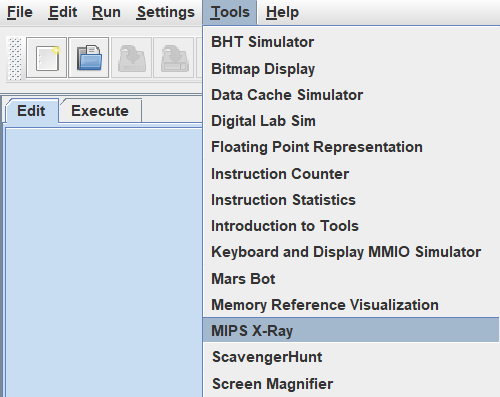
\includegraphics[width=0.7\textwidth]{figura1.png} % Reemplaza en Overleaf
    \caption{Menú Tools de MARS mostrando la opción MIPS X-Ray para la visualización del camino de datos}
\end{figure}


En la ventana que se abre, haga clic en el botón Connect to MIPS para vincular la visualización con el simulador.

Ejecute el programa paso a paso utilizando los botones Step Into.

Al llegar a una instrucción tipo R (por ejemplo,add \$t0, \$s1, \$s2;), el camino de datos se actualizará automáticamente, destacando con colores las rutas activas:

 Lectura de los dos registros fuente (rs y rt) desde el banco de registros.

 Paso de los operandos a la ALU.

 Operación realizada en la ALU (suma, en el caso de add).

 Escritura del resultado en el registro de destino (rd).

 Señales de control activas (RegDst, ALUSrc, RegWrite, etc.).

La herramienta muestra de forma animada o resaltada los componentes involucrados (Instruction Memory, Register File, ALU, MUX, etc.) y las señales de control específicas para instrucciones R-type, permitiendo distinguir claramente el flujo de datos respecto a otros formatos (I-type, J-type, load/store).


\begin{figure}[H]
    \centering
    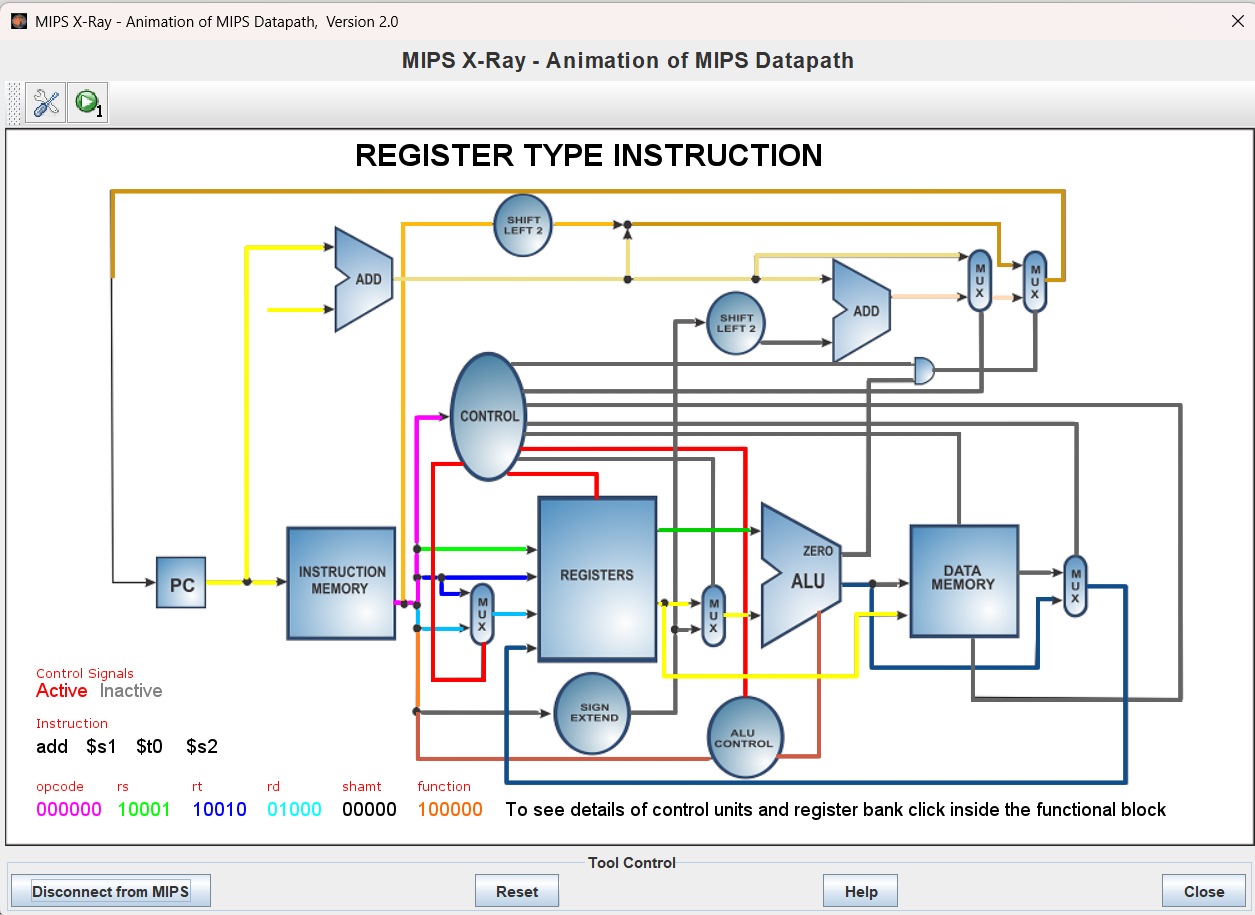
\includegraphics[width=0.9\textwidth]{figura2.png} % Reemplaza en Overleaf
    \caption{Ejecución paso a paso de una instrucción add en la visualización MIPS X-Ray, donde se resaltan en color las señales de control y el flujo de datos a través de las unidades funcionales.}
\end{figure}


Esta visualización resulta especialmente útil para comprender el funcionamiento interno de instrucciones como add, sub, and, or o slt, ya que resalta el camino típico de las instrucciones tipo R y ayuda a identificar cómo interactúan las unidades funcionales en cada ciclo de reloj.

Esta herramienta complementa de manera excelente la ventana de Registros y la ejecución paso a paso, ofreciendo una perspectiva gráfica y educativa del camino de datos que facilita la comprensión del comportamiento a nivel de hardware de los algoritmos implementados.\newpage

\section*{13.¿Cómo puede visualizarse en MARS el camino de datos para una instrucción tipo I? (por ejemplo: lw).}

Una vez conocida la herramienta MIPS X-Ray y el procedimiento general para su activación y conexión con el simulador, el camino de datos de una instrucción tipo I (como lw) se visualiza de manera diferenciada al ejecutar el código paso a paso. Al detenerse en una instrucción de este formato, la representación gráfica resalta un flujo característico que involucra el valor inmediato y el acceso a memoria, a diferencia del recorrido exclusivamente entre registros de las instrucciones tipo R.


\begin{figure}[H]
    \centering
    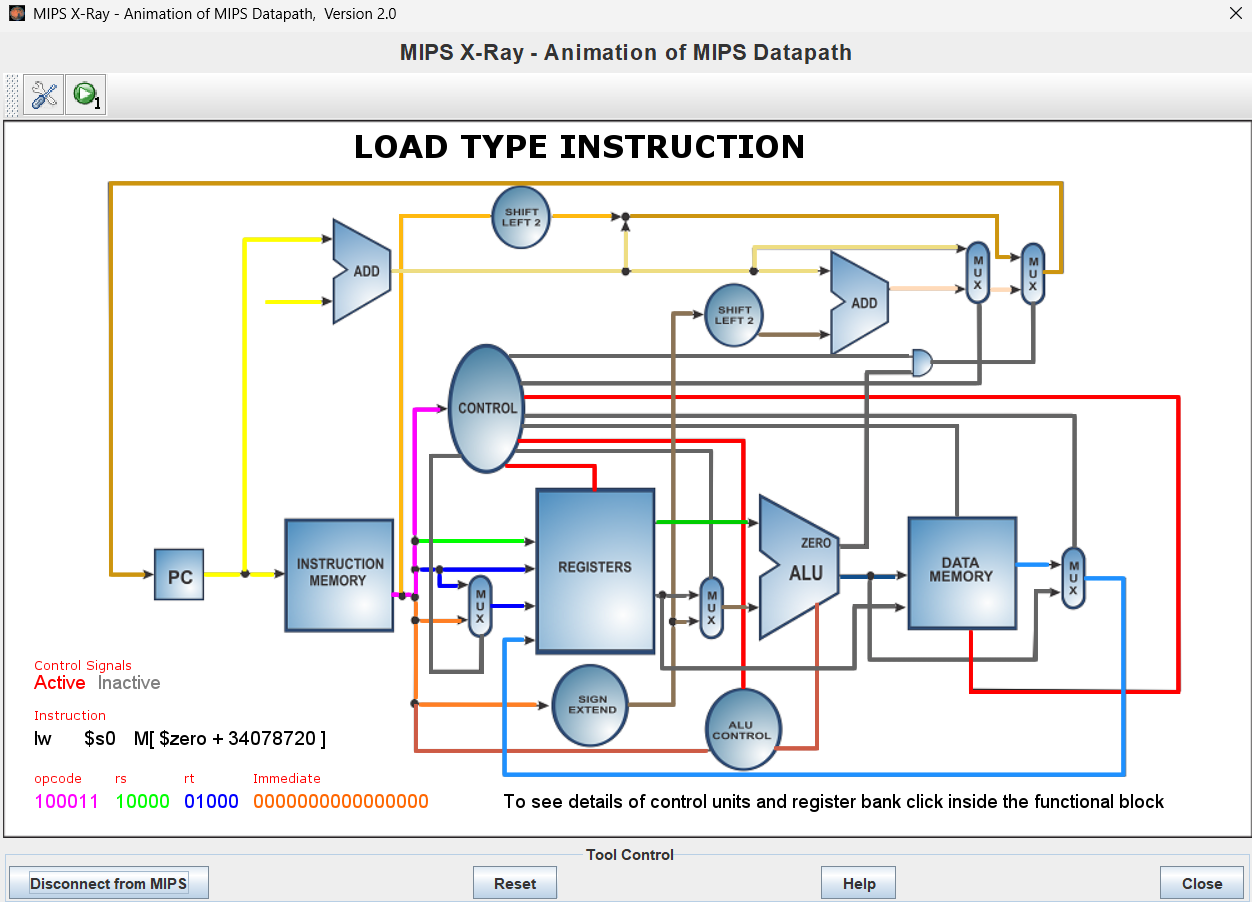
\includegraphics[width=0.9\textwidth]{figura3.png} % Reemplaza en Overleaf
    \caption{Ejecución paso a paso de una instrucción lw en la visualización MIPS X-Ray, donde se resaltan en color las señales de control y el flujo de datos a través de las unidades funcionales[cite: 1].}
\end{figure}


En particular, para lw se observan con claridad las siguientes etapas activas:

Lectura del registro base desde el banco de registros.

Extensión de signo del campo inmediato (offset).

Cálculo de la dirección efectiva mediante la ALU (registro base + valor inmediato extendido).

Acceso a la memoria de datos para la lectura del valor.

Escritura del dato recuperado en el registro de destino.

Estas rutas, destacadas mediante colores específicos, permiten apreciar de forma precisa el modelo load/store de la arquitectura MIPS y comprender cómo una instrucción de carga interactúa con la memoria. Esta visualización resulta especialmente pertinente para analizar las operaciones lw presentes en los algoritmos de ordenamiento implementados, donde se recuperan los elementos del arreglo desde las posiciones de memoria correspondientes.

De esta manera, MIPS X-Ray facilita no solo la observación individual de cada formato de instrucción, sino también la comparación visual entre ellos, enriqueciendo el análisis del comportamiento interno del procesador durante la ejecución de los programas.\newpage

\section*{14.Justificar la elección del algoritmo alternativo.}

Se seleccionó el algoritmo Mergesort (en su versión iterativa) como algoritmo alternativo al Quicksort, debido a un conjunto de características técnicas, pedagógicas y de rendimiento que lo convierten en un complemento ideal para el análisis comparativo en el contexto de la práctica.

En primer lugar, Mergesort ofrece una complejidad temporal garantizada de O(n log n) tanto en el mejor, promedio como en el peor de los casos, esta propiedad resulta especialmente valiosa frente a Quicksort, cuya complejidad puede degradarse hasta O(n²) en situaciones desfavorables (por ejemplo, cuando el arreglo se encuentra ya ordenado o parcialmente ordenado y la elección del pivote no es óptima). Al implementar ambos algoritmos en ensamblador MIPS, es posible observar de forma concreta cómo la predictibilidad de Mergesort se traduce en un comportamiento más estable del número de instrucciones ejecutadas y del uso de la pila, aspecto que no siempre se mantiene en la versión recursiva de Quicksort.

En segundo lugar, la estabilidad del algoritmo (preserva el orden relativo de elementos con valores iguales) aporta un valor adicional desde el punto de vista teórico y práctico, aunque en la práctica se trabajó con números enteros simples, esta característica permite ilustrar un criterio de calidad que Quicksort no garantiza de forma natural, enriqueciendo la discusión sobre las propiedades de los algoritmos de ordenamiento.

Desde el punto de vista de la implementación en ensamblador, Merge Sort iterativo presenta ventajas didácticas relevantes, ya que al ser una versión iterativa, evita la profundidad de recursión que caracteriza a Quicksort, lo que reduce el riesgo de desbordamiento de pila y permite un control más explícito del uso de registros y del arreglo auxiliar (aux). Esto facilita la observación, mediante las herramientas de depuración de MARS (ventana de registros, ejecución paso a paso y MIPS X-Ray), del flujo de datos en las fases de fusión y de la interacción entre memoria principal y registros, además, el uso de un espacio auxiliar de tamaño fijo permite analizar de manera clara el compromiso entre tiempo y espacio).

Por otra parte, la estructura de Merge Sort, basada en la división sucesiva de bloques de tamaño creciente (1, 2, 4, 8…), se alinea de forma natural con el modelo load/store de MIPS y con el uso intensivo de instrucciones tipo I (lw, sw) y tipo R (add, slt), esto posibilita una comparación directa y enriquecedora con las operaciones de partición e intercambio propias de Quick Sort, evidenciando cómo distintas estrategias algorítmicas se traducen en patrones de acceso a memoria y de utilización de la ALU.

Finalmente, la elección de Mergesort como alternativa responde a un criterio formativo: permite al estudiante contrastar dos paradigmas clásicos del diseño de algoritmos (divide y conquista con partición in-place versus divide y conquista con fusión y espacio auxiliar), fortaleciendo la comprensión de las ventajas y limitaciones de cada enfoque cuando se implementan a bajo nivel. De esta manera, no solo se cumple el objetivo de ordenar un arreglo, sino que se genera un espacio de reflexión sobre eficiencia, estabilidad, uso de recursos y comportamiento del procesador MIPS.

En resumen, Mergesort fue seleccionado como algoritmo alternativo por su complejidad temporal predecible, su estabilidad, su implementación iterativa favorable para el análisis en ensamblador y su capacidad de complementar de forma significativa el estudio de Quicksort, ofreciendo una visión más completa de las estrategias de ordenamiento en el contexto de la arquitectura RISC de MIPS.\newpage
\section*{15. Análisis y Discusión de los Resultados}

La implementación de los algoritmos Quicksort y Mergesort en ensamblador MIPS32 permitió evidenciar de forma concreta la estrecha relación entre las decisiones de diseño a bajo nivel y el comportamiento real del procesador, a partir de la observación detallada del uso de registros, del tráfico de memoria, de las estructuras de control y de la complejidad computacional, se desprenden varios hallazgos relevantes que se discuten a continuación.

En primer lugar, la aplicación rigurosa de la convención de llamada de MIPS demostró ser un factor determinante para la correcta ejecución de ambos programas; la distinción entre registros temporales (\$t0–\$t9) y registros guardados (\$s0–\$s7) no constituyó un simple formalismo, sino una necesidad práctica. En particular, el uso de registros guardados para variables de larga duración (como la cantidad de elementos, los límites de los subarreglos o el índice del pivote) garantizó la integridad de los datos a través de las múltiples llamadas a subrutinas y de la recursión, de la misma manera, cuando fue necesario preservar valores ubicados en registros temporales (como ocurrió en la función partition alrededor de la llamada a swap), se debió gestionar manualmente su protección en la pila. Este comportamiento confirma que la convención de registros es una convención de software cuya violación exige un esfuerzo adicional por parte del programador.

Asimismo, el análisis del uso de los registros de argumentos (\$a0–\$a3), de retorno (\$v0) y de dirección de retorno (\$ra) reveló diferencias estructurales entre ambos algoritmos, debido a que Mergesort, al requerir tres límites además de la base del arreglo para la fusión, consumió los四个 registros de argumento disponibles, mientras que Quicksort operó cómodamente con tres, recordando que la protección sistemática de \$ra en todas las funciones que realizan llamadas internas evitó la pérdida de la dirección de retorno, aspecto crítico en un entorno recursivo como el de Quicksort.

Desde el punto de vista del rendimiento, se observó que el principal factor diferenciador no es el acceso inevitable a memoria para leer y escribir los elementos del arreglo, sino el tráfico adicional generado por cada algoritmo; el Quicksort concentra este tráfico en la gestión de la pila asociada a la recursión, cuyo consumo crece con la profundidad de las llamadas y, en el peor caso, puede aproximarse a un comportamiento lineal respecto a n, en cambio, Mergesort, al ser iterativo, mantiene una profundidad de pila constante, pero introduce un costo espacial fijo mediante el arreglo auxiliar. Esta compensación entre espacio y estabilidad temporal se hizo evidente al analizar los marcos de pila y el número de accesos a memoria por comparación.

Las estructuras de control también mostraron impactos diferenciados; en Quicksort la repetición se logra mediante la recursión, de modo que el costo de control se concentra en las fronteras de las llamadas a función (jal/jr y el correspondiente manejo de pila). Por el contrario, en Mergesort, la anidación de bucles (ciclo\_tam, ciclo\_izq y ciclo\_merge) desplaza ese costo hacia un mayor número de instrucciones aritméticas y de comparación dentro de los cuerpos de los bucles. En ambos casos, el uso intensivo de saltos (beq, bne, j y jal) introduce riesgos de control propios de la arquitectura segmentada de MIPS, cuyo efecto se multiplica en los bucles más frecuentemente ejecutados.

En cuanto a la complejidad computacional, los resultados confirman las propiedades teóricas de cada algoritmo puesto que Quicksort mantiene un rendimiento promedio de O(n log n), pero su caso peor O(n²) se traduce, en el entorno MIPS32, en un riesgo real de desbordamiento de pila cuando el arreglo se encuentra ordenado o parcialmente ordenado y el pivote elegido genera particiones desbalanceadas, por otra parte, Mergesort, al dividir por posición y no por valor, garantiza O(n log n) en todos los escenarios y una profundidad de pila predecible, a costa del espacio auxiliar. Esta diferencia resulta especialmente significativa en ensamblador, donde no existen mecanismos automáticos de protección frente al desbordamiento de pila.

Continuando, el modelo RISC de MIPS demostró ser especialmente adecuado para la implementación de ambos algoritmos gracias a la simplicidad y la uniformidad de las instrucciones de longitud fija, el modelo load/store y la disponibilidad de 32 registros de propósito general facilitaron la codificación clara y eficiente de las operaciones críticas de comparación, cálculo de direcciones, acceso a memoria e intercambio, estas características se reflejaron tanto en la partición recursiva de Quicksort como en las fusiones iterativas de Mergesort.

En este aspecto, la depuración sistemática realizada con el modo de ejecución paso a paso (Step y Step Into) y la ventana de Registros de MARS constituyó un pilar fundamental para validar la corrección de los programas, estas herramientas permitieron inspeccionar en tiempo real el estado de los registros, la pila y la memoria de datos, detectando y corrigiendo errores lógicos relacionados con índices, manejo de parámetros y equilibrio de la pila. Complementariamente, la visualización del camino de datos mediante MIPS X-Ray ofreció una perspectiva gráfica del flujo interno del procesador, diferenciando claramente el recorrido registro-registro de las instrucciones tipo R del recorrido que involucra valor inmediato y acceso a memoria propio de las instrucciones tipo I.

Entre diferencias de algoritmos, la elección de Mergesort como algoritmo alternativo se justificó por su complejidad temporal garantizada de O(n log n) en todos los casos, su estabilidad y su naturaleza iterativa, que evita el riesgo de desbordamiento de pila asociado a la recursión profunda de Quicksort, permitiendo contrastar dos paradigmas clásicos de diseño y analizar de forma comparativa el uso de registros, el tráfico de memoria y el comportamiento de la pila en un entorno de bajo nivel.

Finalmente, las pruebas experimentales confirmaron la robustez de ambas implementaciones, se evaluaron arreglos de tamaños 10, 25, 50 y hasta 100 elementos, incluyendo valores grandes y números negativos. En todos estos casos ambos algoritmos produjeron el vector ordenado de forma correcta, sin errores de ejecución. 

Únicamente se observó un comportamiento erróneo cuando no se ingresaba ningún elemento, lo que pone de manifiesto la necesidad de validar previamente el tamaño del arreglo, evidenciando que las implementaciones respetan adecuadamente los límites de memoria reservada y manejan correctamente tanto valores positivos como negativos.

En conjunto, los hallazgos demuestran que la eficiencia y la fiabilidad de un algoritmo de ordenamiento en MIPS32 no dependen únicamente de su complejidad asintótica, sino de la interacción concreta entre el uso de registros, el tráfico de memoria, las estructuras de control y las características de la arquitectura RISC. La comparación entre Quicksort y Mergesort, respaldada por las pruebas realizadas, ilustra de manera clara los compromisos inherentes al diseño a bajo nivel y refuerza la importancia de comprender la arquitectura subyacente al momento de implementar soluciones en ensamblador.

\end{document}\begin{figure}
    \centering
    \includegraphics[width=0.5\linewidth]{Captura de pantalla 2026-07-30 212216.png}
    \caption{Enter Caption}
    \label{fig:placeholder}
\end{figure}
